\documentclass[presentation]{beamer}
\usepackage{../oop-slides-casadei}
\setbeamertemplate{bibliography item}[text]
\newcommand{\lessonnr}[0]{10}
\title[OOP10 -- DVCS Workflow and Lambdas]{10\\ Workflow per DVCS \\ Lambda expression e Stream}

\begin{document}

\frame[label=coverpage]{\titlepage}

%====================
%Outline
%====================
\begin{frame}<beamer>
 	\frametitle{Outline}
 	\tableofcontents[]
\end{frame}



\section{DVCS Workflow}

\subsection{Introduzione}

\fr{Dalle puntate precedenti} {
	\bl{DVCS} {
		\iz {
			\item DVCS sono strumenti potenti per tenere traccia in maniera efficiente della storia di un progetto
			\item Nascono in particolare come evoluzione dei tradizionali VCS (SVN, CVS \dots) 
			\item Enfasi su una \textbf{miglior gestione del lavoro di team}
		}
	}
	\bl{DVCS e teamwork} {
		\iz {
			\item ``La potenza \`e nulla senza controllo!'' 
			\item Ovvero \dots la mancanza di un metodo chiaro e condiviso per utilizzarli può portare a risultati \textbf{DEVASTANTI} 
            \iz {
                \item effort necessario per la parte di gestione diventa presto preponderante e insostenibile            
            }
			\item Ecco perch\'e nella pratica quotidiana, \`e bene adottare un \textbf{workflow collaborativo}
            \iz {
                \item i vostri progetti e i vostri partner di progetto vi ringrazieranno!            
            }
		}
    }
}

\fr{DVCS Workflow} {
	\bl{Cos'è} {
        \iz {
			\item E' una sorta di ``protocollo'', un insieme di regole e passi da seguire quando si utilizza un DVCS
			\item Essendo \textbf{collaborativo} by definition, ciascun team member vi partecipa con un \textbf{ruolo}
			\item Associa le diverse fasi del ciclo di vita del software a una serie di attività
            \iz {
                \item Ogni ruolo ha la/le proprie attività, ognuna codificata in un insieme di passi da seguire         
            }
		}
		
	}
	\bl{Come deve essere} {
		\iz {
			\item In tre aggettivi
            \iz {
                \item Semplice
                \item Chiaro
                \item Condiviso          
            }
		}
    }
}

\subsection{Caratteristiche di un workflow}

\fr{L'importanza dei ruoli} {
        \iz {
			\item Occupandosi di team collaboration, è naturale che il workflow definisca dei ruoli
			\item Nei progetti del ``mondo reale'' il set minimo di ruoli è composto da:
            \iz{
                \item i \textbf{developer}: sviluppano codice, implementano nuove funzionalità, bugfixing di funzionalità già rilasciate

                \item il \textbf{team leader}: coordina l'attività dei developer, sviluppa egli stesso (spesso si prende carico degli aspetti più delicati)

                \item il \textbf{release manager}: si occupa di gestire i rilasci, ovvero ``pubblicazione'' delle nuove funzionalità del software, rese così disponibili ai suoi utenti
            }
		}	
}

\fr{Le attività coperte} {
        \iz {
			\item Sono quelle tipiche del cosiddetto \emph{software lifecycle}
            \iz{
                \item Sviluppo del software (delle nuove funzionalità)

                \item Rilascio delle nuove funzionalità (dopo opportuni test funzionali)

                \item Fix di bug riscontrati nelle versioni già rilasciate (a seguito di segnalazioni da parte degli utenti)
            }
            \item Versioni? Cioè?
		}	
}

\fr{Le versioni} {
        \iz {
			\item Ogni rilascio del software è caratterizzato da una versione, identificata da un \textbf{numero}
            \item il numero ha (o dovrebbe) avere un senso, non è un numero estratto a sorte!
            \item Il pattern tipico è: \textbf{X.Y.Z} (numeri naturali)
            \iz{
                \item \textbf{X - major version}. Identifica una evoluzione importante del software, nella quale funzionalità precedenti possono in generale aver subito modifiche o essere state eliminate.
                    \iz{
                        \item Retrocompatibilità non garantita!                    
                    } 
                \item \textbf{Y - minor version}. Identifica rilasci che aggiungono nuove funzioni, senza toccare quelle già presenti. 
                    \iz{
                        \item Retrocompatibilità garantita!                    
                    } 
                \item \textbf{Z - bugfix version}. Identifica la risoluzione di difetti su una certa release \emph{X.Y}, senza aggiunta, modifica e/o cancellazione di funzionalità
                    \iz{
                        \item Retrocompatibilità garantita!                    
                    } 
            }
            \item Un buon riferimento è: \url{http://semver-ftw.org/}
		}	
}

\fr{Quale workflow} {
        \iz {
			\item Come si sceglie un workflow?
            \item Abbiamo parlato di semplicità...
            \item In realtà è più corretto parlare di giusto \textbf{trade-off} tra semplicità ed esigenze
		}	
}

\subsection{Due esempi di workflow}

\fr{Lo stato dell'arte I} {
%Definito da \emph{Vincent Driessen} e spiegato in \url{http://nvie.com/posts/a-successful-git-branching-model/}
\begin{center}
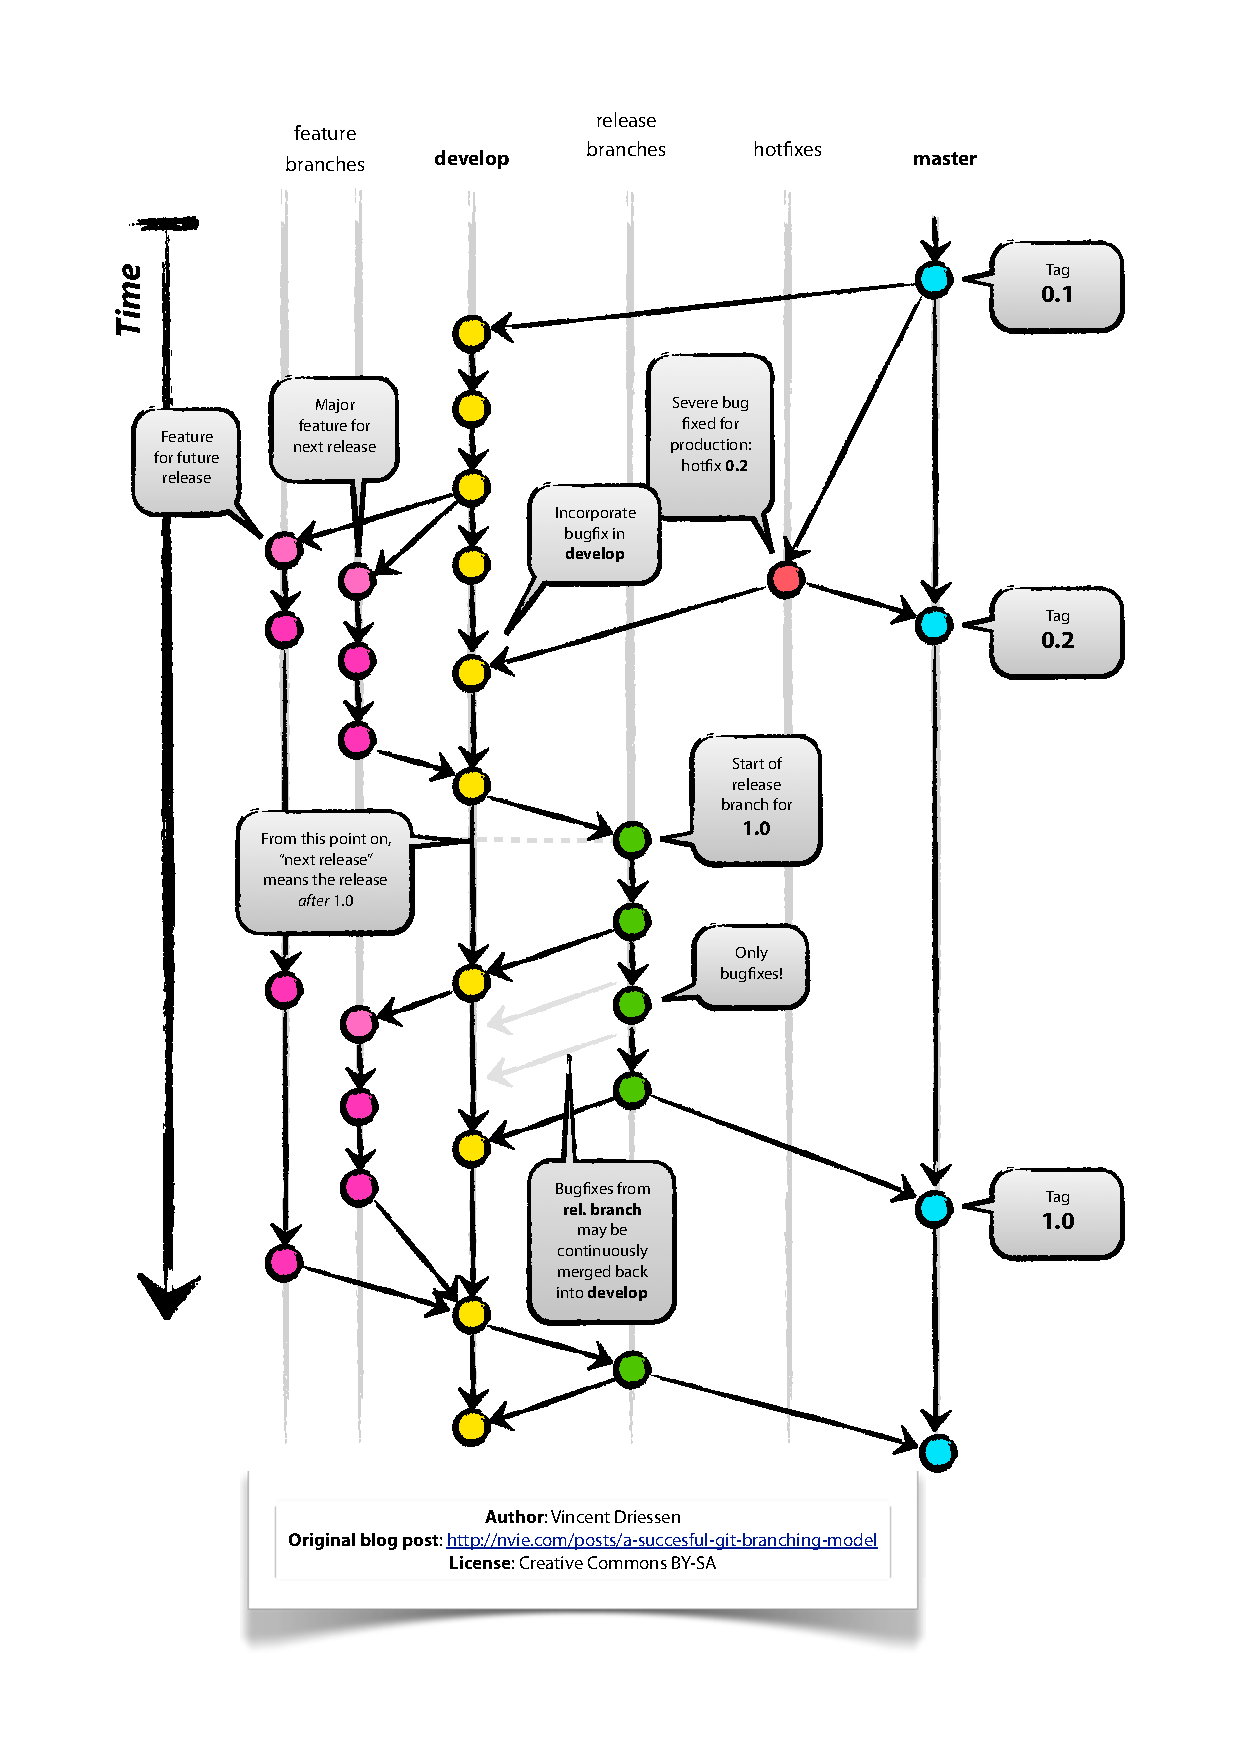
\includegraphics[width=0.5\textwidth]{img/Git-branching-model}
\end{center}
}

\fr{Lo stato dell'arte II} {
    \bl{Alcune considerazioni} {    
        \iz {
            \item Pensato per GIT (ma adottabile anche su Mercurial)
			\item Non lo useremo
            \iz{
                \item troppo complicato per i nostri scopi            
            }
            \item Comunque molto interessante perché racchiude tutti gli aspetti di un DVCS workflow
        }
    }

    \bl{Le branch} {
		\iz {
			\item Sono il supporto fondamentale alle fasi del ciclo di vita del software 
			\item Ogni fase la propria branch! 
			\item Forking e merging di branch sono all'ordine del giorno!
		}
	}
}


\fr{Un modello più semplice} {
\begin{center}
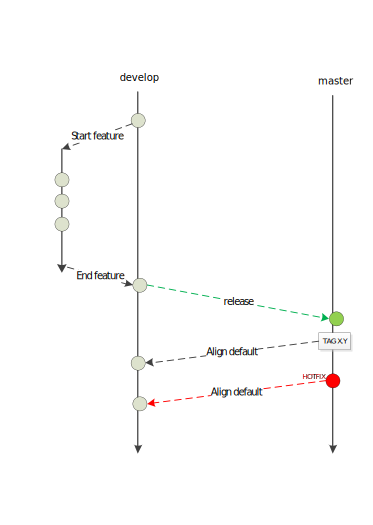
\includegraphics[width=0.5\textwidth]{img/visio-workflow-mercurial}
\end{center}
}

\fr{Rivediamo ruoli e compiti} {
\iz{
\item Developer: 
    \begin{enumerate}
        \item aprono una nuova \textbf{feature branch} da default ogni volta che cominciano lo sviluppo di nuova funzionalità
        \item le \textbf{feature} in realtà si aprono solo per funzionalità ``grandi'', altrimenti si lavora su default
        \item effettuano commit regolari sulla feature branch
        \item terminato lo sviluppo della funzionalità effettuano la merge della feature in default
        \item si occupano anche degli hotfix
    \end{enumerate}

\item Technical leader (per i vostri progetti questa figura non esisterà, probabilmente): 
    \begin{enumerate}
        \item supervisiona la qualità del codice prodotto
        \item è responsabile della qualità del codice che finisce sulla default branch       
    \end{enumerate}

\item Release manager:
    \begin{enumerate}
        \item effettua i rilasci
        \item quando una nuova versione è pronta per il rilascio, effettua il merge della default in stable 
        \item effettua il tagging della release
    \end{enumerate}
}
}

\fr{Sulle feature branch} {
        \iz {
			\item Ha senso utilizzarle per funzionalità/task grandi
            \item In particolare in termini di tempo richiesto per completare l'implementazion
            \item Quando l'attività di analisi abbia già portato ad una classificazione accurata delle funzionalitàe
            \item Per progetti articolati consente di separare e gestire meglio le attività di sviluppo
            \iz{
                \item chi fa cosa
                \item più sviluppatori impegnati sulla stessa funzionalità/task usano la stessa branch            
            }
            \item In contesti articolati può quindi aiutare a tener traccia dello stato di avanzamento di determinate attività
            \item Per i vostri progetti potrebbe non essere così sensato... 
		}	
}

\subsection{Comandi Mercurial}

\fr{Init del repo} {
\sizedcode{\tiny}{code/init.txt}
}

\fr{Uso di una feature} {
\sizedcode{\tiny}{code/open-feature.txt}
}

\fr{Fare una release} {
\sizedcode{\tiny}{code/do-release.txt}
}

\fr{Hotfix} {
\sizedcode{\tiny}{code/hotfix.txt}
}

\fr{E la collaborazione?} {
\iz{
    \item Finora abbiamo mostrato comandi che si eseguono su un singolo repo
    \item Vi ricordate come si fa per condividere gli sviluppi con il resto del vostro team?
    \iz{
        \item clone
        \item push
        \item pull    
    }
    \item E' quindi necessario avere un repository remoto ufficiale per il vostro progetto! $\rightarrow$ BitBucket!
}
}

\fr{Il repo ufficiale del vostro progetto} {
\iz{
    \item Qualcuno di voi agirà come ``repo maintainer''
    \item Creerà quindi il repo su BitBucket
    \item I membri del team eseguiranno quindi:
    \iz{
        \item hg clone URI\_TO\_OFFICIAL\_REPO   
    }
    \item Le attività verranno quindi eseguite sul repo locale (working copy) di ciascun membro del team, con condivisione via official repo tramite \texttt{push} e \texttt{pull}
}
}

\fr{Best practice per la condivisione I} {
Developer
\iz{
    \item In generale, push regolare delle proprie modifiche su repo ufficiale (e pull regolare di quanto presente in remoto)
    \iz{
        \item Se il push riguarda la default branch: le modifiche che condividete via push \textbf{devono compilare}!
    }
    \item Eseguire sempre un pull e update tutte le volte che cominciate a lavorare su qualche cosa in una certa branch 
    \item Per eventuali feature branch? Stesse regole di default (possiamo rilassare qualche vincolo)
    \item Spesso per questioni di revisione del codice e quality check non sempre gli sviluppatori hanno il permesso di fare push direttamente su default
    \iz{
        \item Si può gestire richiedendo una ``pull-request'' sul vs. sistema di hosting (e.g. BitBucket). 
        \item Non ritenuto di particolare utilità per la gestione dei vostri progetti
    } 
    \item Stable non si tocca!
        \iz{
        \item Meglio non garantire i diritti di scrittura (pushing) su stable agli sviluppatori!
    } 
}

}

\fr{Best practice per la condivisione II} {

Release manager
\iz{
    \item Pull e update di default prima di cominciare una release
    \item Push di stable e default al termine della release 
}
}







\fr{Per approfondimenti...} {
A complete Mercurial branching strategy:\\

\url{http://draketo.de/light/english/mercurial/complete-branching-strategy}
}
\end{document}

